\chapter{ماتریس‌ها}

\index{ماتریس}

یک \key{ماتریس} مفهومی ریاضی است
که در برنامه‌نویسی متناظر با یک آرایه دوبعدی است. برای مثال،
\[
A = 
 \begin{bmatrix}
  6 & 13 & 7 & 4 \\
  7 & 0 & 8 & 2 \\
  9 & 5 & 4 & 18 \\
 \end{bmatrix}
\]
یک ماتریس با ابعاد $3 \times 4$ است، یعنی
دارای ۳ سطر و ۴ ستون است.
نماد $[i,j]$ به عنصر واقع در سطر $i$ و ستون $j$
در یک ماتریس اشاره دارد.
برای نمونه، در ماتریس بالا،
$A[2,3]=8$ و $A[3,1]=9$ است.

\index{بردار}

حالت خاصی از ماتریس، یک \key{بردار} است
که ماتریسی یک‌بعدی با ابعاد $n \times 1$ است.
برای مثال،
\[
V =
\begin{bmatrix}
4 \\
7 \\
5 \\
\end{bmatrix}
\]
یک بردار است که سه عنصر دارد.

\index{ترانهاده}

\key{ترانهاده} $A^T$ از ماتریس $A$
زمانی به دست می‌آید که سطرها و ستون‌های $A$
جابه‌جا شوند، یعنی $A^T[i,j]=A[j,i]$:
\[
A^T = 
 \begin{bmatrix}
  6 & 7 & 9 \\
  13 & 0 & 5 \\
  7 & 8 & 4 \\
  4 & 2 & 18 \\
 \end{bmatrix}
\]

\index{ماتریس مربعی}

یک ماتریس را \key{ماتریس مربعی} گویند اگر
تعداد سطرها و ستون‌های آن برابر باشد.
برای نمونه، ماتریس زیر یک
ماتریس مربعی است:

\[
S = 
 \begin{bmatrix}
  3 & 12 & 4  \\
  5 & 9 & 15  \\
  0 & 2 & 4 \\
 \end{bmatrix}
\]

\section{عملگرها}

مجموع $A+B$ برای ماتریس‌های $A$ و $B$
زمانی تعریف می‌شود که ابعاد آن‌ها یکسان باشد.
نتیجه ماتریسی است که هر عنصر آن
برابر با مجموع عناصر متناظر
در $A$ و $B$ است.

برای مثال،
\[
 \begin{bmatrix}
  6 & 1 & 4 \\
  3 & 9 & 2 \\
 \end{bmatrix}
+
 \begin{bmatrix}
  4 & 9 & 3 \\
  8 & 1 & 3 \\
 \end{bmatrix}
=
 \begin{bmatrix}
  6+4 & 1+9 & 4+3 \\
  3+8 & 9+1 & 2+3 \\
 \end{bmatrix}
=
 \begin{bmatrix}
  10 & 10 & 7 \\
  11 & 10 & 5 \\
 \end{bmatrix}.
\]

ضرب ماتریس $A$ در مقدار $x$ به این معنی است
که هر عنصر از $A$ در $x$ ضرب می‌شود.
برای مثال،
\[
 2 \cdot \begin{bmatrix}
  6 & 1 & 4 \\
  3 & 9 & 2 \\
 \end{bmatrix}
=
 \begin{bmatrix}
  2 \cdot 6 & 2\cdot1 & 2\cdot4 \\
  2\cdot3 & 2\cdot9 & 2\cdot2 \\
 \end{bmatrix}
=
 \begin{bmatrix}
  12 & 2 & 8 \\
  6 & 18 & 4 \\
 \end{bmatrix}.
\]

\subsubsection{ضرب ماتریس}

\index{ضرب ماتریس}

حاصل‌ضرب $AB$ برای ماتریس‌های $A$ و $B$
زمانی تعریف می‌شود که اندازه $A$ برابر $a \times n$
و اندازه $B$ برابر $n \times b$ باشد، یعنی
تعداد ستون‌های $A$ برابر با تعداد سطرهای $B$ باشد.
نتیجه ماتریسی به ابعاد $a \times b$ است
که عناصر آن با رابطه زیر محاسبه می‌شوند:
\[
AB[i,j] = \sum_{k=1}^n A[i,k] \cdot B[k,j].
\]

ایده اصلی این است که هر عنصر از $AB$
برابر با مجموع حاصل‌ضرب‌های عناصر $A$ و $B$
مطابق تصویر زیر است:

\begin{center}
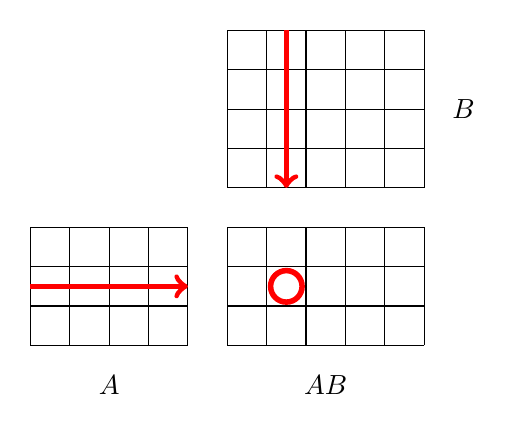
\begin{tikzpicture}[scale=0.5]
\draw (0,0) grid (4,3);
\draw (5,0) grid (10,3);
\draw (5,4) grid (10,8);

\node at (2,-1) {$A$};
\node at (7.5,-1) {$AB$};
\node at (11,6) {$B$};

\draw[thick,->,red,line width=2pt] (0,1.5) -- (4,1.5);
\draw[thick,->,red,line width=2pt] (6.5,8) -- (6.5,4);
\draw[thick,red,line width=2pt] (6.5,1.5) circle (0.4);
\end{tikzpicture}
\end{center}

برای مثال،

\[
 \begin{bmatrix}
  1 & 4 \\
  3 & 9 \\
  8 & 6 \\
 \end{bmatrix}
\cdot
 \begin{bmatrix}
  1 & 6 \\
  2 & 9 \\
 \end{bmatrix}
=
 \begin{bmatrix}
  1 \cdot 1 + 4 \cdot 2 & 1 \cdot 6 + 4 \cdot 9 \\
  3 \cdot 1 + 9 \cdot 2 & 3 \cdot 6 + 9 \cdot 9 \\
  8 \cdot 1 + 6 \cdot 2 & 8 \cdot 6 + 6 \cdot 9 \\
 \end{bmatrix}
=
 \begin{bmatrix}
  9 & 42 \\
  21 & 99 \\
  20 & 102 \\
 \end{bmatrix}.
\]

ضرب ماتریس‌ها شرکت‌پذیر است،
بنابراین $A(BC)=(AB)C$ برقرار است،
اما جابه‌جایی‌پذیر نیست،
بنابراین $AB = BA$ معمولاً برقرار نیست.

\index{ماتریس همانی}

یک \key{ماتریس همانی} ماتریسی مربعی است
که در آن هر عنصر روی قطر اصلی ۱
و تمام عناصر دیگر ۰ هستند.
برای مثال، ماتریس زیر
ماتریس همانی $3 \times 3$ است:
\[
 I = \begin{bmatrix}
  1 & 0 & 0 \\
  0 & 1 & 0 \\
  0 & 0 & 1 \\
 \end{bmatrix}
\]

\begin{samepage}
ضرب یک ماتریس در ماتریس همانی
آن را تغییر نمی‌دهد. برای مثال،
\[
 \begin{bmatrix}
  1 & 0 & 0 \\
  0 & 1 & 0 \\
  0 & 0 & 1 \\
 \end{bmatrix}
\cdot
 \begin{bmatrix}
  1 & 4 \\
  3 & 9 \\
  8 & 6 \\
 \end{bmatrix}
=
 \begin{bmatrix}
  1 & 4 \\
  3 & 9 \\
  8 & 6 \\
 \end{bmatrix} \hspace{10px} \textrm{و} \hspace{10px}
 \begin{bmatrix}
  1 & 4 \\
  3 & 9 \\
  8 & 6 \\
 \end{bmatrix}
\cdot
 \begin{bmatrix}
  1 & 0 \\
  0 & 1 \\
 \end{bmatrix}
=
 \begin{bmatrix}
  1 & 4 \\
  3 & 9 \\
  8 & 6 \\
 \end{bmatrix}.
\]
\end{samepage}

با استفاده از یک الگوریتم سرراست،
می‌توان حاصل‌ضرب دو ماتریس $n \times n$ را
در زمان $O(n^3)$ محاسبه کرد.
الگوریتم‌های کارآمدتری نیز برای ضرب ماتریس‌ها وجود دارند\footnote{نخستین مورد از این الگوریتم‌ها الگوریتم استراسن بود،
منتشر شده در سال ۱۹۶۹ \cite{str69}،
که پیچیدگی زمانی آن $O(n^{2.80735})$ است؛
بهترین الگوریتم فعلی \cite{gal14}
در زمان $O(n^{2.37286})$ کار می‌کند.}،
اما آنها عمدتاً جنبه نظری دارند
و چنین الگوریتم‌هایی در برنامه‌نویسی رقابتی لازم نیستند.


\subsubsection{توان ماتریس}

\index{توان ماتریس}

توان $A^k$ ماتریس $A$ در صورتی تعریف می‌شود
که $A$ یک ماتریس مربعی باشد.
این تعریف مبتنی بر ضرب ماتریس‌ها است:
\[ A^k = \underbrace{A \cdot A \cdot A \cdots A}_{\textrm{$k$ بار}} \]
برای مثال،

\[
 \begin{bmatrix}
  2 & 5 \\
  1 & 4 \\
 \end{bmatrix}^3 =
 \begin{bmatrix}
  2 & 5 \\
  1 & 4 \\
 \end{bmatrix} \cdot
 \begin{bmatrix}
  2 & 5 \\
  1 & 4 \\
 \end{bmatrix} \cdot
 \begin{bmatrix}
  2 & 5 \\
  1 & 4 \\
 \end{bmatrix} =
 \begin{bmatrix}
  48 & 165 \\
  33 & 114 \\
 \end{bmatrix}.
\]
علاوه بر این، $A^0$ ماتریس همانی است. برای مثال،
\[
 \begin{bmatrix}
  2 & 5 \\
  1 & 4 \\
 \end{bmatrix}^0 =
 \begin{bmatrix}
  1 & 0 \\
  0 & 1 \\
 \end{bmatrix}.
\]

ماتریس $A^k$ را می‌توان با استفاده از الگوریتم فصل ۲۱.۲
به‌طور کارآمد در زمان $O(n^3 \log k)$ محاسبه کرد. برای مثال،
\[
 \begin{bmatrix}
  2 & 5 \\
  1 & 4 \\
 \end{bmatrix}^8 =
 \begin{bmatrix}
  2 & 5 \\
  1 & 4 \\
 \end{bmatrix}^4 \cdot
 \begin{bmatrix}
  2 & 5 \\
  1 & 4 \\
 \end{bmatrix}^4.
\]

\subsubsection{دترمینان}

\index{دترمینان}

\key{دترمینان} $\det(A)$ ماتریس $A$
زمانی تعریف می‌شود که $A$ ماتریسی مربعی باشد.
اگر اندازه $A$ برابر $1 \times 1$ باشد،
آن‌گاه $\det(A)=A[1,1]$.
دترمینان ماتریس‌های بزرگ‌تر
به‌صورت بازگشتی با این رابطه محاسبه می‌شود: \index{همساز@همساز (cofactor)}
\[\det(A)=\sum_{j=1}^n A[1,j] C[1,j],\]
که در آن $C[i,j]$ \key{همساز} ماتریس $A$
در سطر $i$ و ستون $j$ است.
همساز از رابطه زیر محاسبه می‌شود:
\[C[i,j] = (-1)^{i+j} \det(M[i,j]),\]
که در آن $M[i,j]$ از حذف سطر $i$
و ستون $j$ ماتریس $A$ به‌دست می‌آید.
به‌دلیل وجود ضریب $(-1)^{i+j}$ در همساز،
علامت دترمینان‌ها یک‌درمیان مثبت
و منفی می‌شود.
برای نمونه،
\[
\det(
 \begin{bmatrix}
  3 & 4 \\
  1 & 6 \\
 \end{bmatrix}
) = 3 \cdot 6 - 4 \cdot 1 = 14 
\]
و
\[
\det(
 \begin{bmatrix}
  2 & 4 & 3 \\
  5 & 1 & 6 \\
  7 & 2 & 4 \\
 \end{bmatrix}
) = 
2 \cdot
\det(
 \begin{bmatrix}
  1 & 6 \\
  2 & 4 \\
 \end{bmatrix}
)
-4 \cdot
\det(
 \begin{bmatrix}
  5 & 6 \\
  7 & 4 \\
 \end{bmatrix}
)
+3 \cdot
\det(
 \begin{bmatrix}
  5 & 1 \\
  7 & 2 \\
 \end{bmatrix}
) = 81.
\]

\index{ماتریس معکوس}

دترمینان $A$ نشان می‌دهد
آیا \key{ماتریس معکوس} $A^{-1}$ وجود دارد
که در رابطه $A \cdot A^{-1} = I$ صدق کند یا خیر؛
که در آن $I$ ماتریس همانی است.
معلوم شده است که $A^{-1}$ دقیقا زمانی وجود دارد
که $\det(A) \neq 0$ باشد،
و می‌توان آن را با فرمول زیر محاسبه کرد:

\[A^{-1}[i,j] = \frac{C[j,i]}{det(A)}.\]

برای نمونه،

\[
\underbrace{
 \begin{bmatrix}
  2 & 4 & 3\\
  5 & 1 & 6\\
  7 & 2 & 4\\
 \end{bmatrix}
}_{A}
\cdot
\underbrace{
 \frac{1}{81}
 \begin{bmatrix}
   -8 & -10 & 21 \\
   22 & -13 & 3 \\
   3 & 24 & -18 \\
 \end{bmatrix}
}_{A^{-1}}
=
\underbrace{
 \begin{bmatrix}
  1 & 0 & 0 \\
  0 & 1 & 0 \\
  0 & 0 & 1 \\
 \end{bmatrix}
}_{I}.
\]

\section{رابطه‌های بازگشتی خطی}

\index{رابطه بازگشتی خطی}

یک \key{رابطه بازگشتی خطی}
تابعی مانند $f(n)$ است
که مقادیر آغازین آن
$f(0),f(1),\ldots,f(k-1)$ بوده
و مقادیر بزرگ‌تر آن
به‌صورت بازگشتی با این رابطه محاسبه می‌شوند:
\[f(n) = c_1 f(n-1) + c_2 f(n-2) + \ldots + c_k f (n-k),\]
که در آن $c_1,c_2,\ldots,c_k$ ضرایب ثابت هستند.

با برنامه‌نویسی پویا می‌توان
هر مقداری از $f(n)$ را در زمان $O(kn)$ با محاسبه
پشت‌سر‌هم مقادیر $f(0),f(1),\ldots,f(n)$ به‌دست آورد.
اما اگر $k$ کوچک باشد، می‌توان
$f(n)$ را با عملیات ماتریسی بسیار کارآمدتر در زمان
$O(k^3 \log n)$ محاسبه کرد.

\subsubsection{اعداد فیبوناچی}

\index{اعداد فیبوناچی}

یک نمونه ساده از رابطه بازگشتی خطی،
تابع زیر است که اعداد فیبوناچی را تعریف می‌کند:
\[
\begin{array}{lcl}
f(0) & = & 0 \\
f(1) & = & 1 \\
f(n) & = & f(n-1)+f(n-2) \\
\end{array}
\]
در این حالت، $k=2$ و $c_1=c_2=1$ است.

\begin{samepage}
برای محاسبه کارآمد اعداد فیبوناچی،
رابطه فیبوناچی را به صورت یک ماتریس مربعی $X$ با اندازه $2 \times 2$
نمایش می‌دهیم که رابطه زیر برای آن برقرار است:
\[ X \cdot
 \begin{bmatrix}
  f(i) \\
  f(i+1) \\
 \end{bmatrix}
=
 \begin{bmatrix}
  f(i+1) \\
  f(i+2) \\
 \end{bmatrix}
 \]
بنابراین، مقادیر $f(i)$ و $f(i+1)$ به عنوان «ورودی» به $X$ داده می‌شوند
و $X$ مقادیر $f(i+1)$ و $f(i+2)$ را از روی آن‌ها محاسبه می‌کند.
چنین ماتریسی برابر است با:

\[ X = 
 \begin{bmatrix}
  0 & 1 \\
  1 & 1 \\
 \end{bmatrix}.
\]
\end{samepage}
\noindent
برای مثال،
\[
 \begin{bmatrix}
  0 & 1 \\
  1 & 1 \\
 \end{bmatrix}
\cdot
 \begin{bmatrix}
  f(5) \\
  f(6) \\
 \end{bmatrix}
=
 \begin{bmatrix}
  0 & 1 \\
  1 & 1 \\
 \end{bmatrix}
\cdot
 \begin{bmatrix}
  5 \\
  8 \\
 \end{bmatrix}
=
 \begin{bmatrix}
  8 \\
  13 \\
 \end{bmatrix}
=
 \begin{bmatrix}
  f(6) \\
  f(7) \\
 \end{bmatrix}.
\]
از این رو، می‌توانیم $f(n)$ را با استفاده از فرمول زیر محاسبه کنیم:
\[
 \begin{bmatrix}
  f(n) \\
  f(n+1) \\
 \end{bmatrix}
=
X^n \cdot
 \begin{bmatrix}
  f(0) \\
  f(1) \\
 \end{bmatrix}
=
 \begin{bmatrix}
  0 & 1 \\
  1 & 1 \\
 \end{bmatrix}^n
\cdot
 \begin{bmatrix}
  0 \\
  1 \\
 \end{bmatrix}.
\]
مقدار $X^n$ در زمان $O(\log n)$ قابل محاسبه است،
بنابراین مقدار $f(n)$ نیز در زمان $O(\log n)$ به دست می‌آید.

\subsubsection{حالت کلی}

اکنون حالت کلی را در نظر می‌گیریم که در آن
$f(n)$ یک رابطه بازگشتی خطی دلخواه است.
هدف دوباره ساخت ماتریس $X$ است به گونه‌ای که:

\[ X \cdot
 \begin{bmatrix}
  f(i) \\
  f(i+1) \\
  \vdots \\
  f(i+k-1) \\
 \end{bmatrix}
=
 \begin{bmatrix}
  f(i+1) \\
  f(i+2) \\
  \vdots \\
  f(i+k) \\
 \end{bmatrix}.
\]
چنین ماتریسی عبارت است از:
\[
X =
 \begin{bmatrix}
  0 & 1 & 0 & 0 & \cdots & 0 \\
  0 & 0 & 1 & 0 & \cdots & 0 \\
  0 & 0 & 0 & 1 & \cdots & 0 \\
  \vdots & \vdots & \vdots & \vdots & \ddots & \vdots \\
  0 & 0 & 0 & 0 & \cdots & 1 \\
  c_k & c_{k-1} & c_{k-2} & c_{k-3} & \cdots & c_1 \\
 \end{bmatrix}.
\]
در $k-1$ سطر اول، هر عنصر برابر 0 است
به جز یک عنصر که 1 است.
این سطرها $f(i)$ را با $f(i+1)$،
$f(i+1)$ را با $f(i+2)$ و به همین ترتیب جایگزین می‌کنند.
سطر آخر شامل ضرایب رابطه بازگشتی برای محاسبه مقدار جدید $f(i+k)$ است.

\begin{samepage}
اکنون، $f(n)$ در زمان $O(k^3 \log n)$ با استفاده از فرمول زیر قابل محاسبه است:
\[
 \begin{bmatrix}
  f(n) \\
  f(n+1) \\
  \vdots \\
  f(n+k-1) \\
 \end{bmatrix}
=
X^n \cdot
 \begin{bmatrix}
  f(0) \\
  f(1) \\
  \vdots \\
  f(k-1) \\
 \end{bmatrix}.
\]
\end{samepage}

\section{گراف‌ها و ماتریس‌ها}

\subsubsection{شمارش مسیرها}

توان‌های ماتریس مجاورت یک گراف ویژگی جالبی دارند.
وقتی $V$ ماتریس مجاورت یک گراف بدون وزن باشد،
ماتریس $V^n$ شامل تعداد مسیرهای به طول $n$ یال بین رأس‌های گراف است.

برای مثال، برای گراف
\begin{center}
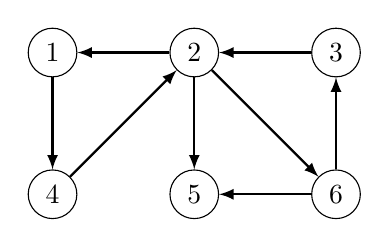
\begin{tikzpicture}[scale=0.9]
\node[draw, circle] (1) at (1,3) {$1$};
\node[draw, circle] (2) at (1,1) {$4$};
\node[draw, circle] (3) at (3,3) {$2$};
\node[draw, circle] (4) at (5,3) {$3$};
\node[draw, circle] (5) at (3,1) {$5$};
\node[draw, circle] (6) at (5,1) {$6$};

\path[draw,thick,->,>=latex] (1) -- (2);
\path[draw,thick,->,>=latex] (2) -- (3);
\path[draw,thick,->,>=latex] (3) -- (1);
\path[draw,thick,->,>=latex] (4) -- (3);
\path[draw,thick,->,>=latex] (3) -- (5);
\path[draw,thick,->,>=latex] (3) -- (6);
\path[draw,thick,->,>=latex] (6) -- (4);
\path[draw,thick,->,>=latex] (6) -- (5);
\end{tikzpicture}
\end{center}
ماتریس مجاورت به صورت زیر است:
\[
V= \begin{bmatrix}
  0 & 0 & 0 & 1 & 0 & 0 \\
  1 & 0 & 0 & 0 & 1 & 1 \\
  0 & 1 & 0 & 0 & 0 & 0 \\
  0 & 1 & 0 & 0 & 0 & 0 \\
  0 & 0 & 0 & 0 & 0 & 0 \\
  0 & 0 & 1 & 0 & 1 & 0 \\
 \end{bmatrix}.
\]
اکنون، برای مثال، ماتریس
\[
V^4= \begin{bmatrix}
  0 & 0 & 1 & 1 & 1 & 0 \\
  2 & 0 & 0 & 0 & 2 & 2 \\
  0 & 2 & 0 & 0 & 0 & 0 \\
  0 & 2 & 0 & 0 & 0 & 0 \\
  0 & 0 & 0 & 0 & 0 & 0 \\
  0 & 0 & 1 & 1 & 1 & 0 \\
 \end{bmatrix}
\]
شامل تعداد مسیرهای با ۴ یال
بین رأس‌ها است.
برای مثال، $V^4[2,5]=2$،
زیرا دو مسیر با ۴ یال
از رأس ۲ به رأس ۵ وجود دارد:
$2 \rightarrow 1 \rightarrow 4 \rightarrow 2 \rightarrow 5$
و 
$2 \rightarrow 6 \rightarrow 3 \rightarrow 2 \rightarrow 5$.

\subsubsection{کوتاه‌ترین مسیرها}

با استفاده از ایده‌ای مشابه در یک گراف وزن‌دار،
می‌توان برای هر جفت از رأس‌ها کمینه طول مسیری
بین آن‌ها را که دقیقاً شامل $n$ یال است محاسبه کرد.
برای محاسبه این مقدار، باید ضرب ماتریسی را
به روشی جدید تعریف کنیم تا به جای محاسبه تعداد
مسیرها، طول مسیرها را کمینه کنیم.

\begin{samepage}
به عنوان مثال، گراف زیر را در نظر بگیرید:
\begin{center}
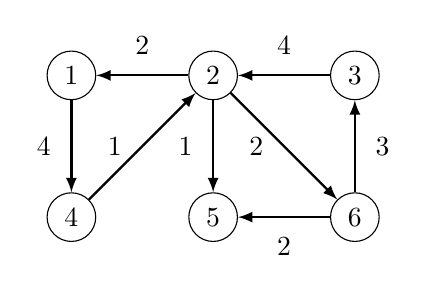
\begin{tikzpicture}[scale=0.9]
\node[draw, circle] (1) at (1,3) {$1$};
\node[draw, circle] (2) at (1,1) {$4$};
\node[draw, circle] (3) at (3,3) {$2$};
\node[draw, circle] (4) at (5,3) {$3$};
\node[draw, circle] (5) at (3,1) {$5$};
\node[draw, circle] (6) at (5,1) {$6$};

\path[draw,thick,->,>=latex] (1) -- node[font=\small,label=left:4] {} (2);
\path[draw,thick,->,>=latex] (2) -- node[font=\small,label=left:1] {} (3);
\path[draw,thick,->,>=latex] (3) -- node[font=\small,label=north:2] {} (1);
\path[draw,thick,->,>=latex] (4) -- node[font=\small,label=north:4] {} (3);
\path[draw,thick,->,>=latex] (3) -- node[font=\small,label=left:1] {} (5);
\path[draw,thick,->,>=latex] (3) -- node[font=\small,label=left:2] {} (6);
\path[draw,thick,->,>=latex] (6) -- node[font=\small,label=right:3] {} (4);
\path[draw,thick,->,>=latex] (6) -- node[font=\small,label=below:2] {} (5);
\end{tikzpicture}
\end{center}
\end{samepage}

ماتریس مجاورتی تشکیل می‌دهیم که در آن
$\infty$ به معنای نبود یال است
و سایر مقادیر نشان‌دهنده وزن یال‌ها هستند.
ماتریس عبارت است از:
\[
V= \begin{bmatrix}
  \infty & \infty & \infty & 4 & \infty & \infty \\
  2 & \infty & \infty & \infty & 1 & 2 \\
  \infty & 4 & \infty & \infty & \infty & \infty \\
  \infty & 1 & \infty & \infty & \infty & \infty \\
  \infty & \infty & \infty & \infty & \infty & \infty \\
  \infty & \infty & 3 & \infty & 2 & \infty \\
 \end{bmatrix}.
\]

به جای فرمول
\[
AB[i,j] = \sum_{k=1}^n A[i,k] \cdot B[k,j]
\]
اکنون از فرمول
\[
AB[i,j] = \min_{k=1}^n A[i,k] + B[k,j]
\]
برای ضرب ماتریس‌ها استفاده می‌کنیم؛ یعنی به جای جمع
کمینه را حساب می‌کنیم
و به جای ضرب مقادیر، مجموع آن‌ها را به دست می‌آوریم.
پس از این تغییر،
توان‌های ماتریس متناظر با
کوتاه‌ترین مسیرها در گراف خواهند بود.

برای نمونه، با توجه به اینکه
\[
V^4= \begin{bmatrix}
  \infty & \infty & 10 & 11 & 9 & \infty \\
  9 & \infty & \infty & \infty & 8 & 9 \\
  \infty & 11 & \infty & \infty & \infty & \infty \\
  \infty & 8 & \infty & \infty & \infty & \infty \\
  \infty & \infty & \infty & \infty & \infty & \infty \\
  \infty & \infty & 12 & 13 & 11 & \infty \\
 \end{bmatrix},
\]
می‌توان نتیجه گرفت که کمینه طول یک مسیر
با ۴ یال
از رأس ۲ به رأس ۵ برابر ۸ است.
یک نمونه از چنین مسیری
$2 \rightarrow 1 \rightarrow 4 \rightarrow 2 \rightarrow 5$
است.

\subsubsection{قضیه کیرشهف}

\index{Kirchhoff's theorem}
\index{spanning tree}

\key{قضیه کیرشهف}
%\footnote{G. R. Kirchhoff (1824--1887) was a German physicist.}
روشی ارائه می‌دهد
تا تعداد درخت‌های پوشای
یک گراف را با استفاده از دترمینان یک ماتریس خاص محاسبه کنیم.
به عنوان مثال، گراف
\begin{center}
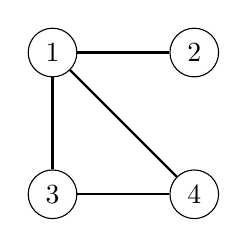
\begin{tikzpicture}[scale=0.9]
\node[draw, circle] (1) at (1,3) {$1$};
\node[draw, circle] (2) at (3,3) {$2$};
\node[draw, circle] (3) at (1,1) {$3$};
\node[draw, circle] (4) at (3,1) {$4$};

\path[draw,thick,-] (1) -- (2);
\path[draw,thick,-] (1) -- (3);
\path[draw,thick,-] (3) -- (4);
\path[draw,thick,-] (1) -- (4);
\end{tikzpicture}
\end{center}
دارای سه درخت پوشا است:
\begin{center}
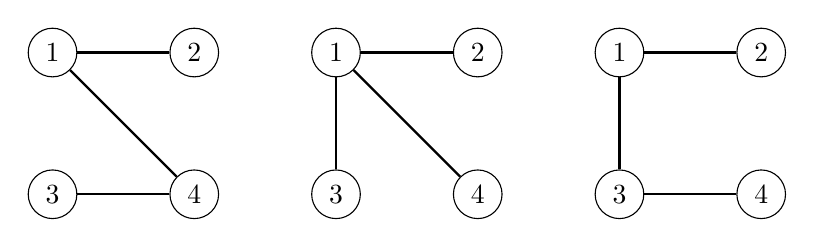
\begin{tikzpicture}[scale=0.9]
\node[draw, circle] (1a) at (1,3) {$1$};
\node[draw, circle] (2a) at (3,3) {$2$};
\node[draw, circle] (3a) at (1,1) {$3$};
\node[draw, circle] (4a) at (3,1) {$4$};

\path[draw,thick,-] (1a) -- (2a);
%\path[draw,thick,-] (1a) -- (3a);
\path[draw,thick,-] (3a) -- (4a);
\path[draw,thick,-] (1a) -- (4a);

\node[draw, circle] (1b) at (1+4,3) {$1$};
\node[draw, circle] (2b) at (3+4,3) {$2$};
\node[draw, circle] (3b) at (1+4,1) {$3$};
\node[draw, circle] (4b) at (3+4,1) {$4$};

\path[draw,thick,-] (1b) -- (2b);
\path[draw,thick,-] (1b) -- (3b);
%\path[draw,thick,-] (3b) -- (4b);
\path[draw,thick,-] (1b) -- (4b);

\node[draw, circle] (1c) at (1+8,3) {$1$};
\node[draw, circle] (2c) at (3+8,3) {$2$};
\node[draw, circle] (3c) at (1+8,1) {$3$};
\node[draw, circle] (4c) at (3+8,1) {$4$};

\path[draw,thick,-] (1c) -- (2c);
\path[draw,thick,-] (1c) -- (3c);
\path[draw,thick,-] (3c) -- (4c);
%\path[draw,thick,-] (1c) -- (4c);
\end{tikzpicture}
\end{center}
\index{ماتریس لاپلاس}
برای محاسبه تعداد درخت‌های فراگیر،
یک \key{ماتریس لاپلاس} $L$ می‌سازیم،
به طوری که $L[i,i]$ درجه رأس $i$ است
و اگر یالی بین رئوس $i$ و $j$ وجود داشته باشد $L[i,j]=-1$،
و در غیر این صورت $L[i,j]=0$ است.
ماتریس لاپلاس برای گراف بالا به شکل زیر است:
\[
L= \begin{bmatrix}
  3 & -1 & -1 & -1 \\
  -1 & 1 & 0 & 0 \\
  -1 & 0 & 2 & -1 \\
  -1 & 0 & -1 & 2 \\
 \end{bmatrix}
\]

می‌توان نشان داد که
تعداد درخت‌های فراگیر برابر است با
دترمینان ماتریسی که از حذف
هر سطر و هر ستون دلخواه از $L$ به دست می‌آید.
برای مثال، اگر سطر و ستون اول را حذف کنیم،
نتیجه برابر است با:

\[ \det(
\begin{bmatrix}
  1 & 0 & 0 \\
  0 & 2 & -1 \\
  0 & -1 & 2 \\
 \end{bmatrix}
) =3.\]
مقدار دترمینان همواره یکسان است،
صرف‌نظر از اینکه کدام سطر و ستون از $L$ حذف شود.

توجه کنید که فرمول کیلی در بخش ۲۲.۵ یک
حالت خاص از قضیه کیرشهف است،
زیرا در یک گراف کامل با $n$ رأس داریم:

\[ \det(
\begin{bmatrix}
  n-1 & -1 & \cdots & -1 \\
  -1 & n-1 & \cdots & -1 \\
  \vdots & \vdots & \ddots & \vdots \\
  -1 & -1 & \cdots & n-1 \\
 \end{bmatrix}
) =n^{n-2}.\]